\chapter{Introduction}
\label{chap:introduction}

%Zooming in part of the introduction
Software development is a notoriously error-prone process, and writing a program of a certain size without errors is infeasible. A major part of software development is therefore concerned with finding bugs and eliminating them. Testing is widely used as a technique to detect bugs, but the programmer never knows whether the absence of failed test cases means a missing test case, or that the software is free of errors. Writing an appropriate set of test cases can be very challenging, and running them can be a time-consuming process. It is especially difficult to write exhaustive test cases for concurrent systems, e.g., for a communication protocol where several process instances are executing at the same time.

Building an abstract representation of the system in form of a \emph{model} is another way to detect bugs. The model can be used to verify properties in a system, e.g., that a system does not contain any deadlocks, or that a communication protocol behaves correct in an unreliable network. In Fig.~\ref{fig:specmodelimpl} we show a typical way of using models in software development. The model is build on the basis of a system specification written in plain English. After verifying that the model has the desired properties, it can be used as a basis of an implementation. 

\begin{figure}[h!]
\centering
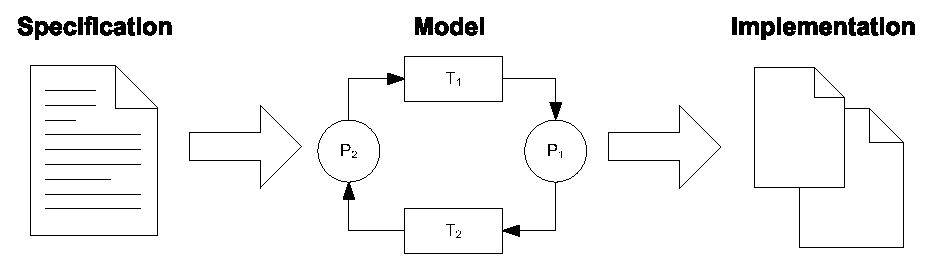
\includegraphics[scale=0.7]{introduction/graphics/spec_model_impl_figure.eps}
\caption{Phases in software development using models}
\label{fig:specmodelimpl}
\end{figure}

%Formal verification advantages
The advantage of constructing a model in the development phase is at least threefold: 
\begin{itemize}
\item Developers are forced to be precise about essential parts of the specification in the process of building the model. Specifications are often ambiguous because they are written in plain English, and details may be missing in the specification. Finding these errors early in the development process can save a lot of resources later.

\item By using the appropriate tools it is possible to perform simulations of a model. A simulation is very similar to an execution of a program. It shows how the model behaves in different situations which can be used to debug the specification. 

\item From a model it is possible to generate a state space, which is a directed graph, where states are represented as nodes and events \ignore{, that changes the system to a new state, }are represented as arcs. The state space can be explored in order to mathematically prove that the system has a given property. This is important in systems were an error can have catastrophic consequences, e.g., in the software controlling the cooling system of a reactive core in a nuclear power plant. 
\end{itemize}

% State space analysis disadvantages
A problem with state space analysis is that the number of states a system can reach often grow rapidly when the model becomes more complex. This is known as the \emph{state explosion problem} \cite{Val98}, and is a big challenge when performing state space exploration. It is often possible to restrict the model, or build the state space partially and still find errors in the system. 

% Translating the model to code
Another problem with the approach shown in Fig.~\ref{fig:specmodelimpl} is that there may be a mismatch between the specification, the model, and the actual implementation. This is because the translation: specification $\rightarrow$ model $\rightarrow$ imhhhplementation is done manually, and hence errors may be introduced in each step of the translation. A way to reduce this problem is to use the model as the specification and automatically generate the implementation from the model. The details abstracted away in the model will of course also lack in the implementation, but eliminating errors in the important parts of the system would lead to more reliable software with fewer errors. \ignore{and could save a lot of resources compared to making the translation manually.}\\

% Example to motivate automatic code generation
Network protocols are an example of why automatic code generation is useful in software development. The \underline{Dy}namic \underline{M}ANET \underline{O}n-demand (DYMO) Routing Protocol \cite{refWorks:69} is a protocol for routing in mobile ad-hoc networks. The Internet Draft describing the protocol is currently at version 16 and about to become an Internet Standard. The specification is written in English describing the different operations of the protocol, and it can be used as a basis for an implementation. Because natural language specifications are often ambiguous translating them to either an implementation or a model requires that the developer make some choices. These choices can make the implementation flawed, and it can also make interoperability between different implementation difficult. 

Specifying DYMO as a formal model (instead of plain English) would exclude ambiguities in the specification. It would also make it easier to directly find errors or verify properties of the specification. In an earlier project \cite{RefWorks:6} we showed, that a model of the DYMO protocol containing all the mandatory parts can be constructed using relatively few resources. The problem is that manually implementing the protocol based on the model may introduce errors, and it would therefore be better \ignore{and more cost-efficient} to generate most of the implementation automatically. In the case of the DYMO protocol, technical details like packet formats and configurations are abstracted away in the model, so they would have to be implemented manually. But the protocol logic and the structure of the implementation would be generated automatically and therefore preserving the behaviour of model in the code.


\section{Coloured Petri Nets}

Petri nets \cite{Petri} is an executable graphical modelling language represented by a bi-graph consisting of nodes and arcs. It can be used to describe a discrete-event concurrent system. An example of such a concurrent system could be a communication protocol. A model could be used to analyse whether it is possible to bring the protocol in an undesirable state, e.g., a deadlock. Nodes in a Petri net are either transitions representing discrete events, or places representing conditions. Arcs in a Petri net describe the pre- and post-condition relation between transitions. 

% Coloured Petri Nets
Coloured Petri Nets (CP-nets or CPNs) \cite{RefWorks:3} is a high-level Petri net language, i.e., the Petri net formalism with added high-level programming functionalities. The programming language used is CPN ML which is based on the general-purpose functional programming language Standard ML \cite{RefWorks:67}. CPN ML provides support for commonly used functionality, e.g., defining data types and manipulating data. Every part of the CPN language has a formal definition, i.e., it is defined mathematically what will happen, e.g., when events occur in the model. This makes it possible to simulate an execution of a CPN model to inspect which states the model can reach. 

CPN Tools \cite{RefWorks:3} is a graphical CPN editor in which it is possible to construct and simulate CPN models. Through the graphical user interface the user can construct a model and do step-by-step simulation. This is much easier than constructing and simulating the CPN model according to the mathematical definition by hand.

When performing a simulation of a model, only one possible execution of the system is explored. But often it is interesting to look at every possible execution of the system to analysis whether it is possible for the model to reach an undesirable state. As mentioned, this can be done by generating and exploring the state space of the model to analyse the behaviour of the system. There exist a range of tools that suppot state space exploration. CPN Tools has built-in support for generating and exploring state spaces. Another computer tool is the \underline{A}SCoVeCo \underline{S}tate space \underline{A}nalysis \underline{P}latform (ASAP) \cite{RefWorks:92}. ASAP is a platform that supports state space analysis of CPN models using state-of-the-art exploration algorithms. The program is built on top of the Eclipse Rich Client platform \cite{RefWorks:73} which makes is very easy to extend, a fact we take advantage of later in this thesis.

\section{Code Generation}
An often used definition of code generation is one computer program producing another computer program in an automatic way. A well known type of code generator is a compiler, e.g., Sun's javac \cite{refWorks:70} or GNU's GCC \cite{refWorks:71}. A compiler typically takes a human-readable text file as input and outputs an executable program. The produced program is often low-level code, e.g., machine code.

The type of code generation presented in this thesis is \emph{source code generation}. The input to this kind of code generator is a formal model specified for instance in a graphical modelling language, and the output is human-readable source code written in a high-level programming language. A compiler has the advantage that high-level programming languages are designed such that the translation into low-level code always makes sense and has equivalent behaviour. Source code generation from a formal model do not have the same advantage. A model is an abstraction of a system and because of the generality of the model it is often very hard to obtain equivalent behaviour in the source code.

Also, the level of abstraction has to be taken into consideration. In one model the focus might be on the details of packet transmission in a network, whereas in another model these details might have been abstracted away. This can make it hard to generate code since it is difficult to make an interpretation of the structures in the model.

\section{Thesis Aims and Results}
The aim of this thesis is to develop a technique to automatically generate code from CPN models. The code should be readable and intuitive such that the user can read, modify and extend the generated code. We also require that the model should be clearly recognizable in the generated code since the people working with the generated code would typically be very familiar with the model. The technique should allow different target languages to be used, e.g., C, Java, SML or Erlang. However the target language should be invisible in the model and the usual inscription language should be used in the model.

We achieved the aim by defining a subclass of CP-nets called Process-Partitioned CP-nets (ProPCP-nets or ProPCPNs). ProPCPN models preserve most of the general-purpose strength of CP-nets as we show by constructing a model of the advanced DYMO protocol. We have developed a technique that translates from the class of ProPCP-nets to the Erlang programming language, and created an implementation of the technique as a proof of concept. The implementation is able to generate readable code from the DYMO model, and we validate that the generated code has the same behaviour as the model. 


\ignore{
%% OLD AIM:
%% Model: Restriction vs. expressiveness, target language invisible
Our aim is to define a subclass of CP-nets which preserves the general-purpose strength of CP-nets, but enables us to generate code for the models in the class. To show the expressive power of the class we construct a model of the complex communication protocol DYMO in this class. Our focus in the translation is more on generating readable code than on generating high performance code. It is for instance more important that the programmer is able to recognize the model in the code than making the code highly optimised.

%% Tool
As a proof of concept we implement a tool which given a CPN model in our subclass of CPNs generates an Erlang source code implementation of the model. The implementation should have the same behaviour and properties as the model.

}

\section{Thesis Outline}
The structure of the thesis is described below. The thesis is written in close cooperation between the two authors, but as required we have divided the responsibility of the chapters. 

\begin{description}
\item[Chapter~\ref{chap:background}~\nameref{chap:background}] In this chapter we establish the background for understanding the thesis. We present the CPN model of a producer-consumer system which is the running example throughout the thesis. We also present the target language of the translation, namely Erlang, and describe the basic constructs of the Erlang language. Kristian is responsible for Sec.~\ref{sec:cpn}, and Mads is responsible for Sec.~\ref{sec:erlang}. 

\item[Chapter~\ref{chap:codegeneration}~\nameref{chap:codegeneration}] Different approaches to code generation is discussed on the basis of related work. We illustrate some of the approaches using manually translated code examples, and discuss advantages and disadvantages. Mads is responsible for this chapter.

\item[Chapter~\ref{chap:netclass}~\nameref{chap:netclass}] ProPCPN is a subclass of CPN that we constructed to generate code from, and we give an intuitive description as well as a formal definition of the net class. We also show that the producer-consumer model presented in chapter~\ref{chap:background} fits into this subclass. Mads is responsible for this chapter.

\item[Chapter~\ref{chap:translation}~\nameref{chap:translation}] In this chapter we present a technique to generate Erlang source code from ProPCPN models. We present all the phases of the translation, and use the simple producer-consumer model to illustrate the translation. Mads is responsible Sec.~\ref{sec:cpntodcpn}, Sec.~\ref{sec:dcpntocfg}, and Sec.~\ref{sec:cfgtoast}. Kristian is responsible for Sec.~\ref{sec:astest}, Sec.~\ref{sec:esttocode}, and Sec.~\ref{sec:advancedissues}.

\item[Chapter~\ref{chap:tool}~\nameref{chap:tool}] In this chapter we present our implementation of the translation technique presented in chapter~\ref{chap:translation}. We also validate the code generated from the producer-consumer model. Kristian is responsible for this chapter.

\item[Chapter~\ref{chap:dymo}~\nameref{chap:dymo}] In this chapter we show the expressive power of ProPCPN models by constructing a model of the industrial-sized protocol DYMO. We automatically generate code from the model using our implementation of the translation, and show that the protocol logic from the model is preserved in the generated code. Kristian is responsible for this chapter.

\item[Chapter~\ref{chap:confutwo}~\nameref{chap:confutwo}] Finally, we conclude and summaries on the findings in this thesis and outline some directions for future work.

\end{description}

The implementation of the translation can be found on the enclosed CD-ROM (see appendix \ref{appsec:cd} for more information). The reader is expected to have a basic understanding of formal models, whereas the formal modelling language Coloured Petri Nets is introduced in section \ref{sec:cpn}. Knowledge about SML (or a similar functional language) is also expected, whereas the fundamental concepts of the functional programming language Erlang are explained in section~\ref{sec:erlang}.
